%==================== PARTIE 4 ====================
\section{Partie 4 : Séparation de deux voix par filtrage de Wiener}

\begin{enonce}
\textbf{Énoncé :} Implémenter un filtrage de Wiener sur le mélange $x=d_1+d_2$ pour séparer les deux sources, sur tout le signal puis par trame. Étudier l'effet de l'ordre $P$, de la longueur de trame et du recouvrement. Tracer les performances ($\mathrm{EQM}_{\min,j}$, gain en RSB, qualité perceptuelle PESQ), étudier la robustesse du filtre à la connaissance de $\mathbf{r}_{d_1}$ et envisager d'autres structures (cascade, soustraction, filtrage fréquentiel).
\end{enonce}

\textbf{Le problème.} Dans les parties 2 et 3, le signal à éliminer était un bruit blanc : il occupe toute la bande et ne ressemble pas au signal utile. Ici, le « bruit » est une seconde voix : il est coloré, non stationnaire et occupe la même bande que la voix recherchée. C'est le cas défavorable observé en partie~3~(f) avec le bruit coloré.

\textbf{Formulation.} On calcule un filtre par source. Pour extraire $d_j$ ($j=1,2$) :
\[
\mathbf{R}_x\,\mathbf{w}_j=\mathbf{r}_{d_jx},\qquad \hat d_j(n)=\sum_{k=0}^{P-1}w_j(k)\,x(n-k).
\]
Les deux voix sont indépendantes, donc décorrélées : $r_{d_jx}(k)=r_{d_j}(k)$ et $r_x(k)=r_{d_1}(k)+r_{d_2}(k)$. Dans le domaine fréquentiel (filtre de Wiener RII du cours), le filtre optimal vaut
\[
H_j(e^{j\omega})=\frac{P_{d_jx}(e^{j\omega})}{P_x(e^{j\omega})}=\frac{P_{d_j}(e^{j\omega})}{P_{d_1}(e^{j\omega})+P_{d_2}(e^{j\omega})}.
\]
À chaque fréquence, le filtre garde la part de la puissance qui appartient à $d_j$. Il ne peut donc séparer les voix que là où leurs spectres diffèrent.

\textbf{Critères.} Pour chaque source, $\mathrm{EQM}_{\min,j}=r_{d_j}(0)-\mathbf{w}_j^T\mathbf{r}_{d_j}$ et
\[
\mathrm{gain}_j|_{\mathrm{dB}}=10\log_{10}\frac{P_{d_j}}{\mathrm{EQM}_j}-10\log_{10}\frac{P_{d_j}}{P_{d_{j'}}},
\]
où $d_{j'}$ est l'autre voix, qui joue le rôle du bruit.

\textbf{Signaux.} Deux enregistrements de l'Open Speech Repository~\cite{osr} : une voix d'homme ($d_1$, \texttt{OSR\_us\_000\_0030\_8k.wav}) et une voix de femme ($d_2$, \texttt{OSR\_us\_000\_0010\_8k.wav}), échantillonnées à $F_s=8$~kHz. On garde les $8$ premières secondes ($N=64\,000$), on centre les signaux et on met $d_2$ à la puissance de $d_1$ : le RSB avant séparation vaut $0$~dB pour chaque source. Ce corpus est conçu pour les tests de qualité de la parole, et $8$~kHz est la fréquence de PESQ en bande étroite. Un mélange homme-femme est un cas favorable : les spectres des deux voix diffèrent.

\textbf{Organisation.}
\begin{itemize}
  \item Filtre global : mise en place, cas de référence.
  \item Ordre $P$, traitement par trames, recouvrement de 50~\% : suivre la non-stationnarité de la parole.
  \item Robustesse à la connaissance de $\mathbf{r}_{d_1}$ (dictionnaire par $k$-means), puis proposition originale : filtre de Wiener itératif à modèle AR.
  \item Synthèse avec une mesure de qualité perceptuelle (PESQ), le RSB ne mesurant pas ce que l'on entend ; perspectives (cascade, soustraction, filtrage dans le domaine fréquentiel).
\end{itemize}

\subsection{Filtre global : mise en place et premiers résultats}

\begin{enonce}
\textbf{Objectif :} Calculer un seul filtre de Wiener par source sur tout le signal ($P=10$). C'est le cas de référence de la partie : on observe ce que le filtre exploite (les spectres des deux voix) et ce qu'il obtient.
\end{enonce}

\textbf{Démarche.} La fonction \texttt{separation\_wf} reprend le calcul de la partie~3 avec $d_j$ comme signal de référence et l'autre voix comme bruit. Elle est appelée deux fois, une fois par source. On trace les DSP des deux voix (\texttt{pwelch}) et les réponses en fréquence des deux filtres (\texttt{freqz}).

\textbf{Code.} Fonction de séparation :
\begin{lstlisting}
function [dhat, EQMmin, EQMmes, gain_dB, w] = separation_wf(x, d, b, P)
% Estimation de la source d dans le melange x = d + b par filtre de Wiener
% Entrees : x (melange), d (source cible), b (autre source), P (ordre)
% Sorties : dhat (source estimee), EQM theorique et mesuree, gain en dB, w

x = x(:); d = d(:); b = b(:);

rx = xcorr(x, P-1, 'biased'); rx = rx(P:end);
rd = xcorr(d, P-1, 'biased'); rd = rd(P:end);   % r_dx = r_d (sources decorrelees)
w  = toeplitz(rx) \ rd;              % filtre de Wiener
dhat = filter(w, 1, x);              % source estimee

EQMmin = rd(1) - w'*rd;              % EQM theorique
EQMmes = mean((d - dhat).^2);        % EQM mesuree

% Gain : RSB avant (d face a b) / RSB apres (d face au residu)
RSB_av  = 10*log10(mean(d.^2) / mean(b.^2));
RSB_ap  = 10*log10(mean(d.^2) / EQMmes);
gain_dB = RSB_ap - RSB_av;
end
\end{lstlisting}

Script principal :
\begin{lstlisting}
clear; clc; close all;
dossier = fileparts(mfilename('fullpath'));   % dossier du script
rep = fullfile(dossier, 'figs_partie4', filesep);
if ~isfolder(rep), mkdir(rep); end

%% Chargement des deux voix (Open Speech Repository, 8 kHz)
url = 'https://www.voiptroubleshooter.com/open_speech/american/';
f1  = fullfile(dossier, 'OSR_us_000_0030_8k.wav');   % voix d'homme
f2  = fullfile(dossier, 'OSR_us_000_0010_8k.wav');   % voix de femme
if ~isfile(f1), websave(f1, [url 'OSR_us_000_0030_8k.wav']); end
if ~isfile(f2), websave(f2, [url 'OSR_us_000_0010_8k.wav']); end
[d1, Fs1] = audioread(f1);
[d2, Fs2] = audioread(f2);
d1 = d1(:,1);  d2 = d2(:,1);
if Fs1 ~= Fs2                        % meme frequence d'echantillonnage
    d2 = resample(d2, Fs1, Fs2);
end
Fs = Fs1;

Tmax = 8;                            % duree gardee (s)
N  = min([length(d1), length(d2), round(Tmax*Fs)]);
d1 = d1(1:N);  d2 = d2(1:N);
d1 = d1 - mean(d1);  d2 = d2 - mean(d2);       % sources centrees
d2 = d2 * sqrt(mean(d1.^2) / mean(d2.^2));     % meme puissance -> RSB = 0 dB
x  = d1 + d2;                        % melange

%% Spectres des deux sources
[S1, f] = pwelch(d1, hamming(512), 256, 1024, Fs);
S2      = pwelch(d2, hamming(512), 256, 1024, Fs);
figure;
plot(f, 10*log10(S1), 'b', 'LineWidth', 1.2); hold on;
plot(f, 10*log10(S2), 'r', 'LineWidth', 1.2);
grid on; xlabel('f (Hz)'); ylabel('DSP (dB/Hz)');
legend('d_1 : voix d''homme', 'd_2 : voix de femme');
saveas(gcf, [rep 'p4_q1_dsp.png']);

%% Filtre de Wiener global
P = 10;
[d1h, EQM1, EQMm1, g1, w1] = separation_wf(x, d1, d2, P);
[d2h, EQM2, EQMm2, g2, w2] = separation_wf(x, d2, d1, P);

%% Reponses en frequence des deux filtres
[H1, fh] = freqz(w1, 1, 1024, Fs);
H2       = freqz(w2, 1, 1024, Fs);
figure;
plot(fh, abs(H1), 'b', 'LineWidth', 1.2); hold on;
plot(fh, abs(H2), 'r', 'LineWidth', 1.2);
plot(fh, abs(H1 + H2), 'k--');
grid on; xlabel('f (Hz)'); ylabel('|H(f)|');
legend('|H_1| : extrait d_1', '|H_2| : extrait d_2', '|H_1 + H_2|');
saveas(gcf, [rep 'p4_q1_freqz.png']);

%% Ecoute : melange, puis estimees
sound(x, Fs);    pause(N/Fs + 0.5);
sound(d1h, Fs);  pause(N/Fs + 0.5);
sound(d2h, Fs);
\end{lstlisting}

\begin{figure}[H]
  \centering
  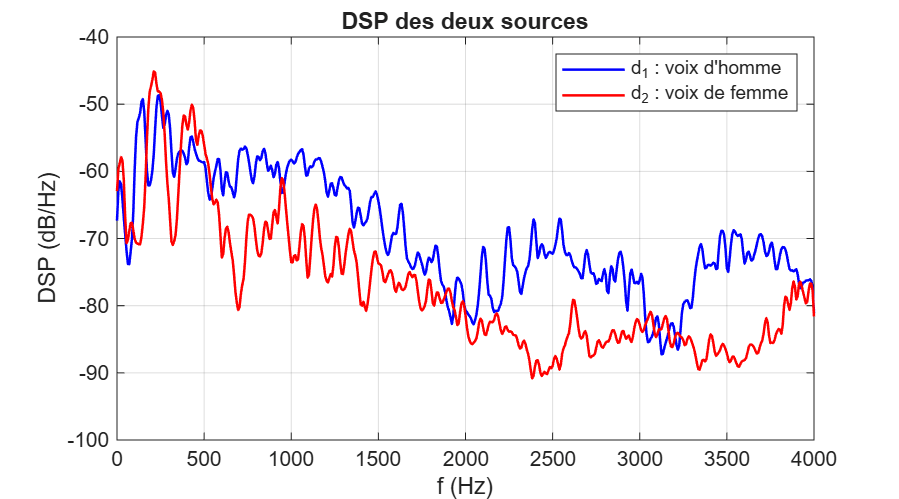
\includegraphics[width=\linewidth]{p4_q1_dsp}
  \caption{DSP de la voix d'homme $d_1$ et de la voix de femme $d_2$ (même puissance).}
\end{figure}

\begin{figure}[H]
  \centering
  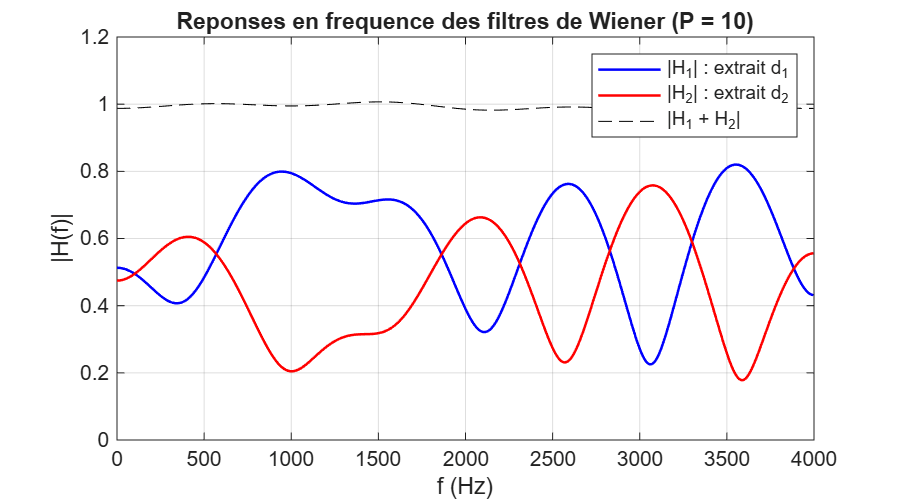
\includegraphics[width=\linewidth]{p4_q1_freqz}
  \caption{Réponses en fréquence des filtres de Wiener globaux ($P=10$) et de leur somme.}
\end{figure}

\begin{resultat}
$P_{d_1}=P_{d_2}=0.0027$. Pour les deux sources : $\mathrm{EQM}_{\min}=\mathrm{EQM}_{\text{mesurée}}=0.0012$, soit un gain de $\mathbf{3.48}$~dB (RSB de $0$ à $3.48$~dB).
\end{resultat}

\begin{interpretation}
\begin{itemize}
  \item \textbf{Qui domine où.} Le filtre ne dépend pas de l'endroit où chaque voix a le plus d'énergie, mais du rapport $P_{d_1}/P_{d_2}$ à chaque fréquence. L'homme domine sous $180$~Hz (son fondamental, entre $100$ et $150$~Hz) et au-dessus de $600$~Hz. La femme domine de $200$ à $500$~Hz, où se trouvent son fondamental ($\approx 200$~Hz) et sa 2\textsuperscript{e} harmonique : à puissance totale égale, elle concentre son énergie sur peu d'harmoniques.
  \item \textbf{Réponses des filtres.} $|H_1|$ est grand là où l'homme domine ($\approx 0.8$ vers $1$~kHz), $|H_2|$ là où la femme domine ($\approx 0.6$ vers $400$~Hz). Les gains restent entre $0.2$ et $0.8$ : le filtre ne coupe aucune fréquence, il pondère. Avec $P=10$ coefficients, sa résolution est grossière ($\approx F_s/P=800$~Hz) : il ne distingue pas la zone de l'homme sous $180$~Hz de celle de la femme entre $200$ et $500$~Hz.
  \item \textbf{$|H_1+H_2|\approx 1$, d'où des gains égaux.} Comme $\mathbf{r}_x=\mathbf{r}_{d_1}+\mathbf{r}_{d_2}$, on a $\mathbf{w}_1+\mathbf{w}_2=\mathbf{R}_x^{-1}\mathbf{r}_x=[1,0,\dots,0]^T$ ($\mathbf{r}_x$ est la première colonne de $\mathbf{R}_x$). Donc $\hat d_1+\hat d_2\approx x$ et $e_2\approx-e_1$ : les deux EQM sont égales, et les gains aussi puisque $P_{d_1}=P_{d_2}$. L'écart à $1$ ($<2$~\%) vient de l'intercorrélation de $d_1$ et $d_2$, non nulle sur une durée finie.
  \item \textbf{Écoute.} Dans $\hat d_1$, l'homme est nettement mis en avant ; dans $\hat d_2$, on entend peu de différence avec le mélange, pour le même gain en RSB. Le résidu d'homme dans $\hat d_2$ se trouve entre $600$ et $4000$~Hz, la zone où l'oreille est la plus sensible (formants, consonnes). Le RSB mesure une puissance d'erreur, pas ce que l'on entend : il faut une mesure perceptuelle comme PESQ.
\end{itemize}
\end{interpretation}

\begin{resultat}[Conclusion]
Le filtre global ne sépare que partiellement les deux voix ($+3.5$~dB) : il ne voit que les spectres moyens sur $8$~s, qui se recouvrent, et $P=10$ est trop faible pour suivre leurs détails. On étudie donc ensuite l'ordre $P$, le traitement par trames et l'évaluation par PESQ.
\end{resultat}

\subsection{Influence de l'ordre \texorpdfstring{$P$}{P} du filtre global}

\begin{enonce}
\textbf{Objectif :} Vérifier si un filtre plus long sépare mieux les deux voix. Avec $P$ coefficients, $H(f)$ ne peut pas former de détail plus étroit qu'environ $F_s/P$ : $800$~Hz pour $P=10$, $160$~Hz pour $P=50$, $40$~Hz pour $P=200$.
\end{enonce}

\textbf{Démarche.} Filtre global (tout le signal, $N=64\,000$), $P$ de $2$ à $200$. Le chargement des voix est regroupé dans une fonction \texttt{charger\_voix(Tmax)} (même code qu'en section précédente).

\textbf{Code.}
\begin{lstlisting}
[d1, d2, x, Fs] = charger_voix(8);

%% Gain du filtre global en fonction de P
Plist = [2 5 10 20 30 50 75 100 150 200];
g1 = zeros(size(Plist));  g2 = zeros(size(Plist));
for m = 1:length(Plist)
    P = Plist(m);
    [~, ~, ~, g1(m)] = separation_wf(x, d1, d2, P);
    [~, ~, ~, g2(m)] = separation_wf(x, d2, d1, P);
end
figure;
plot(Plist, g1, 'bo-', 'LineWidth', 1.3); hold on;
plot(Plist, g2, 'r*--', 'LineWidth', 1.1);
grid on; xlabel('P'); ylabel('gain (dB)');
legend('d_1 : homme', 'd_2 : femme', 'Location', 'southeast');
saveas(gcf, [rep 'p4_q2_gain_P.png']);

%% Reponse en frequence de H1 pour plusieurs P (resolution ~ Fs/P)
Pvis = [10 50 200];
coul = {'b', 'm', 'k'};
figure;
for m = 1:length(Pvis)
    [~, ~, ~, ~, w1] = separation_wf(x, d1, d2, Pvis(m));
    [H1, fh] = freqz(w1, 1, 2048, Fs);
    plot(fh, abs(H1), coul{m}, 'LineWidth', 1.1); hold on;
end
grid on; xlabel('f (Hz)'); ylabel('|H_1(f)|');
legend('P = 10', 'P = 50', 'P = 200');
saveas(gcf, [rep 'p4_q2_H1_P.png']);
\end{lstlisting}

\begin{figure}[H]
  \centering
  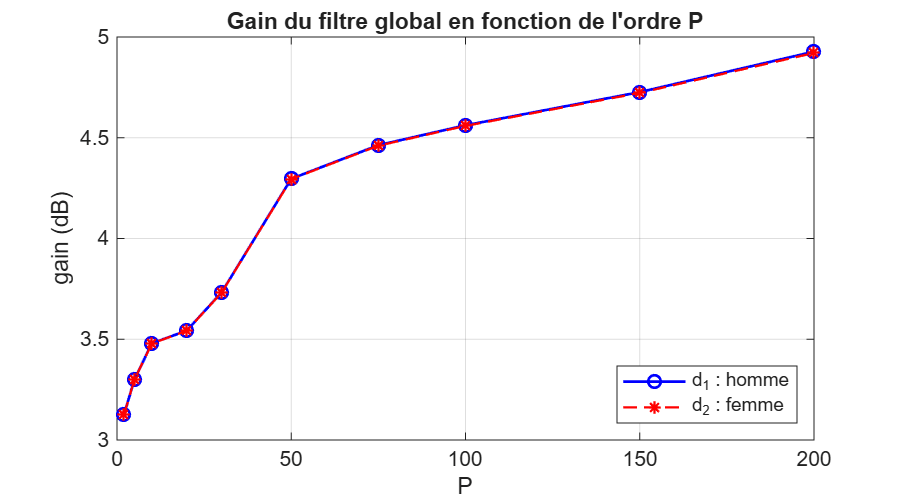
\includegraphics[width=\linewidth]{p4_q2_gain_P}
  \caption{Gain du filtre global en fonction de l'ordre $P$ (les deux courbes sont superposées).}
\end{figure}

\begin{figure}[H]
  \centering
  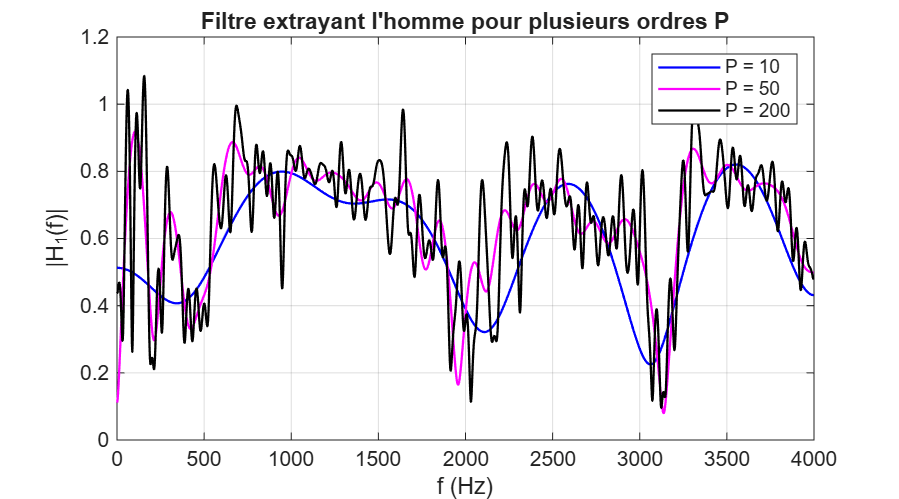
\includegraphics[width=\linewidth]{p4_q2_H1_P}
  \caption{Réponse en fréquence du filtre extrayant l'homme pour $P=10$, $50$ et $200$.}
\end{figure}

\begin{resultat}
Le gain passe de $3.13$~dB ($P=2$) à $3.48$~dB ($P=10$), $3.73$~dB ($P=30$), $\mathbf{4.30}$~dB ($P=50$) puis $4.93$~dB ($P=200$). Les gains des deux voix restent égaux à $0.01$~dB près.
\end{resultat}

\begin{interpretation}
\begin{itemize}
  \item \textbf{Un coude vers $P=50$.} Le saut le plus fort est entre $P=30$ et $P=50$ ($+0.57$~dB pour $20$ coefficients). Au-delà, le gain ne croît plus que lentement ($+0.63$~dB de $50$ à $200$, pour $150$ coefficients).
  \item \textbf{Lecture fréquentielle.} À $P=50$ ($\approx 160$~Hz de résolution), $H_1$ peut enfin suivre l'alternance des zones : $|H_1|\approx 0.9$ vers $100$--$150$~Hz (fondamental de l'homme), $\approx 0.3$ entre $200$ et $500$~Hz (zone de la femme), puis $0.7$--$0.9$ au-dessus. À $P=10$, cette zone était moyennée ($|H_1|\approx 0.4$--$0.5$).
  \item \textbf{Lecture temporelle.} La période fondamentale de la femme vaut $\approx F_s/200 = 40$ échantillons. Avec $P\geq 40$, le filtre couvre une période entière et exploite la périodicité de sa voix. C'est la même condition que $F_s/P\leq F_0$ : résoudre le fondamental en fréquence revient à couvrir une période en temps.
  \item \textbf{Au-delà de $P=50$.} $H_1$ devient très irrégulier à $P=200$ (variations de $0.1$ à $1.08$ sur quelques dizaines de Hz) : il suit les détails fins du spectre moyen. Ces détails sont en partie brouillés, car la hauteur des voix varie sur $8$~s, d'où un gain faible par coefficient ajouté.
  \item \textbf{Comparaison avec la partie~3.} Le coude y était à $P=10$ : contre un bruit blanc, une forme large suffisait. Ici, les deux spectres s'entrecroisent sur quelques centaines de Hz, ce qui demande un filtre plus fin.
\end{itemize}
\end{interpretation}

\begin{resultat}[Conclusion]
$P=50$ est le meilleur compromis pour le filtre global : il résout le fondamental des voix et donne l'essentiel du gain. Même à $P=200$, le gain reste limité ($<5$~dB) : le filtre global ne voit que les spectres moyens. Pour aller plus loin, il faut suivre l'évolution des spectres dans le temps, donc traiter par trames.
\end{resultat}

\subsection{Traitement par trames : longueur de trame et ordre}

\begin{enonce}
\textbf{Objectif :} Recalculer un filtre de Wiener sur chaque trame pour suivre la non-stationnarité de la parole. Sur $20$~ms, les spectres des deux voix diffèrent beaucoup plus qu'en moyenne : souvent, une voix se tait, les deux voix prononcent des sons différents, et la hauteur de chaque voix est stable.
\end{enonce}

\textbf{Le compromis.} L'estimateur biaisé $\hat r(k)=\frac1L\sum_n x(n)x(n-k)$ ne dispose que de $L-k$ produits. Pour une trame de $L=160$ échantillons ($20$~ms), $\hat r(0)$ utilise $160$ produits mais $\hat r(99)$ seulement $61$ (et il est biaisé d'un facteur $61/160$). Une trame courte suit mieux l'évolution des voix, mais impose un ordre $P$ petit devant $L$. Une trame longue estime bien les corrélations, mais revient vers les spectres moyens. Les cas $P>L/2$ ne sont pas calculés.

\textbf{Démarche.} Pour chaque trame (sans recouvrement), $\mathbf{w}_i$ est calculé à partir de $\hat r_x$ et $\hat r_{d_j}$ estimés sur la trame. Comme en partie~3, on utilise le signal propre de chaque trame : c'est le meilleur cas possible, le cas où $\mathbf{r}_{d_1}$ est inconnu est traité plus loin. Chaque trame est filtrée avec les $P-1$ échantillons précédents de $x$, pour que le filtre ne reparte pas d'une mémoire vide. Le gain est calculé sur le signal reconstruit entier. Pour $L=20$~ms et $P=20$, on calcule aussi le RSB avant et le gain de chaque trame où l'homme parle (puissance supérieure à $1$~\% de sa puissance moyenne).

\textbf{Code.} Filtrage par trames :
\begin{lstlisting}
function dhat = separation_trames(x, d, P, L)
% Filtre de Wiener recalcule sur chaque trame de L echantillons (sans recouvrement)
x = x(:); d = d(:);
N = length(x);
K = floor(N / L);                    % nombre de trames
dhat = zeros(N,1);

for i = 1:K
    idx = (i-1)*L+1 : i*L;           % indices de la trame i
    rx = xcorr(x(idx), P-1, 'biased'); rx = rx(P:end);
    rd = xcorr(d(idx), P-1, 'biased'); rd = rd(P:end);
    w  = toeplitz(rx) \ rd;          % filtre de la trame i

    % On filtre avec les P-1 echantillons passes de x (pas de remise a zero)
    deb = max(1, idx(1)-P+1);
    y = filter(w, 1, x(deb:idx(end)));
    dhat(idx) = y(end-L+1:end);
end
end
\end{lstlisting}

Script (extrait) :
\begin{lstlisting}
[d1, d2, x, Fs] = charger_voix(8);
gain = @(d, dh) 10*log10(mean(d.^2) / mean((d - dh).^2));   % RSB_av = 0 dB

%% Gain en fonction de la longueur de trame, pour plusieurs P
Lms   = [5 10 20 40 100 200];        % longueurs de trame (ms)
Plist = [10 20 50];
G1 = nan(length(Plist), length(Lms));  G2 = G1;
for p = 1:length(Plist)
    P = Plist(p);
    for l = 1:length(Lms)
        L = round(Lms(l)*1e-3*Fs);
        if P > L/2, continue; end    % trop peu d'echantillons pour estimer P retards
        G1(p,l) = gain(d1, separation_trames(x, d1, P, L));
        G2(p,l) = gain(d2, separation_trames(x, d2, P, L));
    end
end

%% Criteres par trame (L = 20 ms, P = 20)
P = 20;  L = round(20e-3*Fs);  K = floor(length(x)/L);
d1h = separation_trames(x, d1, P, L);
RSBav = nan(K,1);  g = nan(K,1);
for i = 1:K
    idx = (i-1)*L+1 : i*L;
    p1 = mean(d1(idx).^2);  p2 = mean(d2(idx).^2);
    if p1 < 0.01*mean(d1.^2), continue; end    % homme silencieux : trame ignoree
    RSBav(i) = 10*log10(p1 / p2);
    g(i)     = 10*log10(p1 / mean((d1(idx) - d1h(idx)).^2)) - RSBav(i);
end
\end{lstlisting}

\begin{figure}[H]
  \centering
  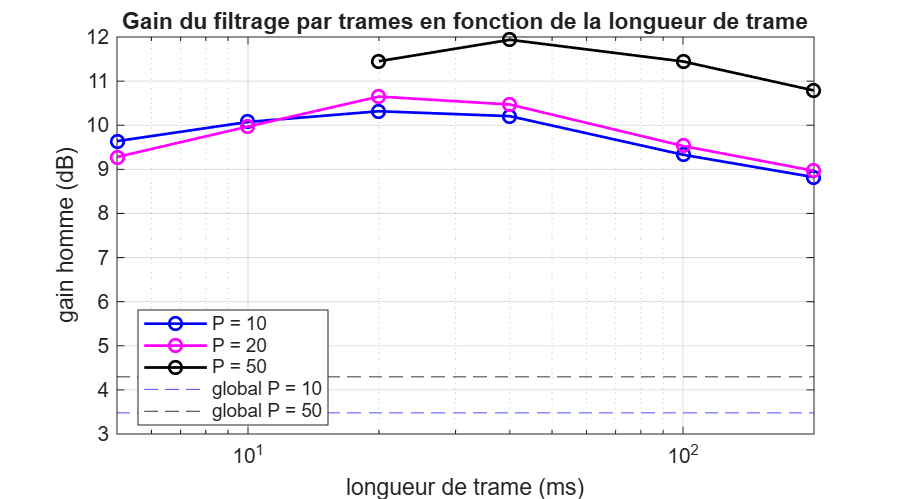
\includegraphics[width=\linewidth]{p4_q3_gain_L}
  \caption{Gain (homme) du filtrage par trames en fonction de la longueur de trame, pour $P=10$, $20$ et $50$. En pointillés : filtre global.}
\end{figure}

\begin{table}[H]
\centering
\small
\begin{tabular}{lcccccc}
\toprule
$L$ (ms) & 5 & 10 & 20 & 40 & 100 & 200 \\
\midrule
$P=10$ & 9.64 & 10.07 & \textbf{10.32} & 10.21 & 9.33 & 8.82 \\
$P=20$ & 9.28 & 9.97 & \textbf{10.65} & 10.47 & 9.53 & 8.97 \\
$P=50$ & -- & -- & 11.45 & \textbf{11.94} & 11.45 & 10.79 \\
\midrule
Global & \multicolumn{6}{c}{$3.48$~dB ($P=10$), $4.30$~dB ($P=50$)} \\
\bottomrule
\end{tabular}
\caption{Gain (dB) de l'homme selon $L$ et $P$. Les gains de la femme sont égaux à $0.6$~dB près.}
\end{table}

\begin{figure}[H]
  \centering
  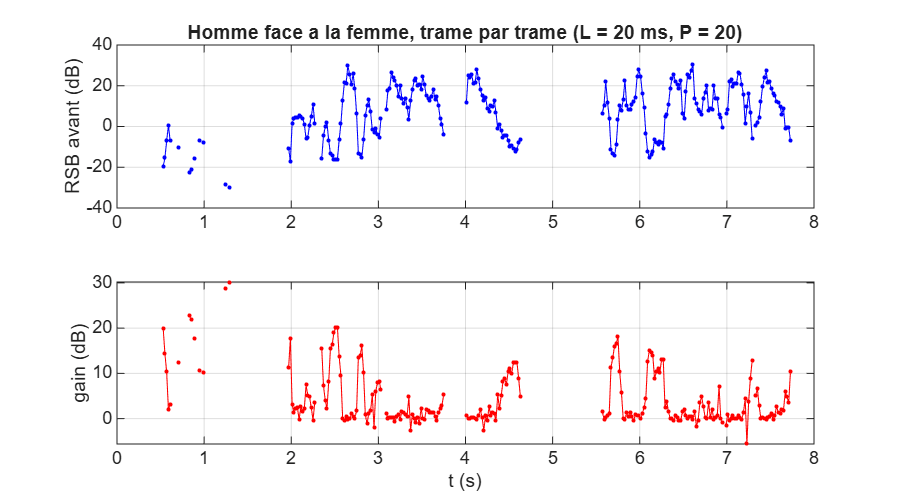
\includegraphics[width=\linewidth]{p4_q3_par_trame}
  \caption{RSB avant (homme face à la femme) et gain de chaque trame où l'homme parle ($L=20$~ms, $P=20$).}
\end{figure}

\begin{figure}[H]
  \centering
  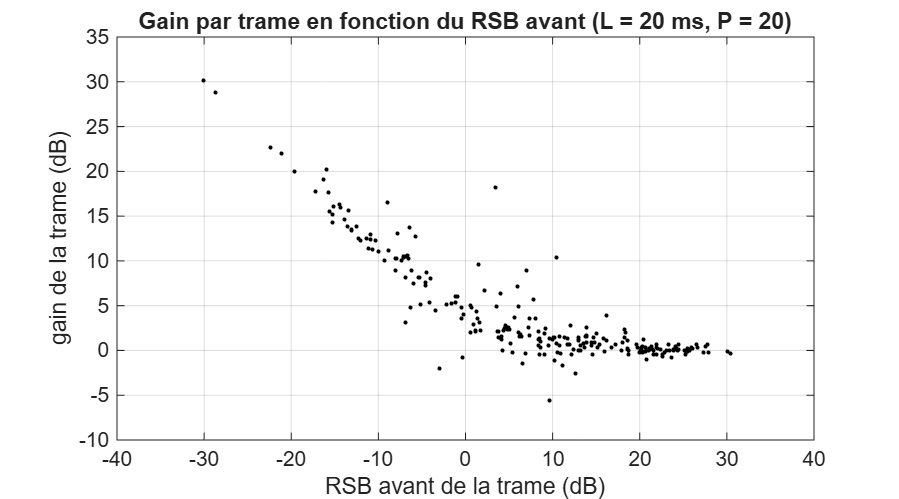
\includegraphics[width=0.85\linewidth]{p4_q3_gain_vs_RSB}
  \caption{Gain de chaque trame en fonction de son RSB avant ($L=20$~ms, $P=20$).}
\end{figure}

\begin{resultat}
Le gain passe de $4.30$~dB (global, $P=50$) à $\mathbf{11.94}$~dB (trames de $40$~ms, $P=50$), soit $+7.6$~dB. À l'écoute, chaque estimée ne contient presque plus que la voix recherchée. Gain moyen par trame ($L=20$~ms, $P=20$, trames où l'homme parle) : $4.29$~dB.
\end{resultat}

\begin{interpretation}
\begin{itemize}
  \item \textbf{Optimum de longueur de trame.} Chaque courbe a un maximum entre $20$ et $40$~ms. Pour des trames courtes, l'estimation des corrélations est bruitée : à $5$~ms ($40$ échantillons), $P=20$ ($=L/2$) fait moins bien que $P=10$. Pour des trames longues, on revient vers les spectres moyens : le gain baisse de $1.2$ à $1.7$~dB entre l'optimum et $200$~ms. L'optimum se déplace vers des trames plus longues quand $P$ augmente ($20$~ms pour $P=10$ et $20$, $40$~ms pour $P=50$) : plus de retards à estimer demande plus d'échantillons.
  \item \textbf{D'où vient le gain.} Trame par trame, le RSB avant varie de $-30$ à $+30$~dB : la plupart du temps, une voix domine nettement. Le filtre se comporte alors presque comme un interrupteur, $\mathbf{w}_i\approx[1,0,\dots,0]^T$ (laisser passer) si la cible domine, $\mathbf{w}_i\approx\mathbf{0}$ (couper) sinon. Même avec $P=10$, dont la résolution en fréquence est grossière, le gain atteint $10$~dB : l'essentiel de la séparation vient de la sélection dans le temps, pas de la forme du spectre.
  \item \textbf{Gain par trame et RSB avant.} Quand l'homme est noyé (RSB avant $<0$), le gain vaut presque $-\mathrm{RSB}_{\mathrm{av}}$ : le filtre coupe la trame, donc $\hat d_1\approx 0$, l'erreur vaut $d_1$ et le RSB après vaut $\approx 0$~dB. La femme est supprimée, mais l'homme n'est pas récupéré. Quand l'homme domine ($>20$~dB), le gain est nul : le filtre laisse tout passer. La vraie séparation spectrale n'a lieu qu'entre $0$ et $10$~dB, avec quelques dB de gain.
  \item \textbf{Gain moyen par trame ($4.29$~dB) et gain global ($10.65$~dB).} La moyenne des gains en dB donne le même poids à chaque trame, et beaucoup de trames où l'homme domine ont un gain proche de $0$. Le gain global compare des énergies totales : il compte aussi les trames où l'homme se tait, que le filtre coupe presque parfaitement, alors que le filtre global laissait passer la femme pendant ces silences. Les deux critères mesurent des choses différentes.
  \item \textbf{Limite.} Ce résultat suppose $\mathbf{r}_{d_1}$ connu sur chaque trame, c'est-à-dire qu'on sait à chaque instant qui parle et avec quel spectre. C'est une borne supérieure ; le cas réaliste est traité dans les sections sur la robustesse.
\end{itemize}
\end{interpretation}

\begin{resultat}[Conclusion]
Le traitement par trames est l'étape décisive : il fait passer le gain d'environ $4$~dB à $10$--$12$~dB, et la séparation devient nette à l'écoute. Le meilleur réglage est une trame de $20$ à $40$~ms avec $P$ petit devant $L$ ($P=50$ et $L=40$~ms ici). Ce gain vient surtout de ce que, sur une trame courte, une voix domine presque toujours l'autre.
\end{resultat}

\subsection{Recouvrement de 50~\% et reconstruction par overlap-add}

\begin{enonce}
\textbf{Objectif :} Sans recouvrement, le filtre change brusquement à chaque frontière de trame ($\mathbf{w}_i$ puis $\mathbf{w}_{i+1}$), ce qui peut créer des sauts dans la sortie. On fait avancer les trames de $L/2$ et on reconstruit le signal par overlap-add, pour passer progressivement d'un filtre au suivant.
\end{enonce}

\textbf{Démarche.} Chaque trame $i$ est filtrée par son propre filtre : $\hat d_1^{\,t_i}=x^{t_i}*\mathbf{w}^i_{opt,1}$. Sa sortie est pondérée par une fenêtre de Hann de longueur $L$, puis ajoutée à la sortie globale. Des fenêtres de Hann décalées de $L/2$ ont une somme égale à $1$ : chaque échantillon de sortie est un mélange des sorties de deux filtres voisins, dont les poids varient progressivement. Les corrélations sont estimées sur la trame non fenêtrée, comme sans recouvrement, pour que seule la reconstruction change. Les discontinuités sont mesurées comme en partie~3 : saut moyen $|\hat d(n+1)-\hat d(n)|$ aux débuts de trame divisé par le saut moyen sur tout le signal ($1$ = pas de discontinuité). Le premier et le dernier $L$ échantillons, où les fenêtres ne se complètent pas, sont exclus du calcul du gain.

\textbf{Code.} Filtrage par trames avec recouvrement et overlap-add :
\begin{lstlisting}
function dhat = separation_ola(x, d, P, L)
% Filtre de Wiener par trames de L echantillons avec recouvrement de 50 %
% et reconstruction par overlap-add (fenetre de Hann, somme des fenetres = 1)
x = x(:); d = d(:);
N   = length(x);
H   = L/2;                           % pas d'avancement : 50 % de recouvrement
win = hann(L, 'periodic');           % fenetres decalees de L/2 : somme = 1
dhat = zeros(N,1);

for s = 1:H:N-L+1
    idx = s : s+L-1;                 % indices de la trame
    rx = xcorr(x(idx), P-1, 'biased'); rx = rx(P:end);
    rd = xcorr(d(idx), P-1, 'biased'); rd = rd(P:end);
    w  = toeplitz(rx) \ rd;          % filtre de la trame

    deb = max(1, s-P+1);             % P-1 echantillons passes de x
    y = filter(w, 1, x(deb:idx(end)));
    y = y(end-L+1:end);
    dhat(idx) = dhat(idx) + win .* y;   % overlap-add
end
end
\end{lstlisting}

Script (extrait) :
\begin{lstlisting}
P   = 20;
Lms = [10 20 40 100];
for l = 1:length(Lms)
    L = round(Lms(l)*1e-3*Fs);
    dh_sr  = separation_trames(x, d1, P, L);
    dh_ola = separation_ola(x, d1, P, L);

    E = L+1 : N-L;                   % on exclut les bords (fenetres incompletes)
    G_sr(l)  = 10*log10(mean(d1(E).^2) / mean((d1(E) - dh_sr(E)).^2));
    G_ola(l) = 10*log10(mean(d1(E).^2) / mean((d1(E) - dh_ola(E)).^2));

    % Saut moyen aux debuts de trame / saut moyen partout (1 = pas de discontinuite)
    df = abs(diff(dh_sr));   S_sr(l)  = mean(df(L:L:end))     / mean(df);
    df = abs(diff(dh_ola));  S_ola(l) = mean(df(L/2:L/2:end)) / mean(df);
end
\end{lstlisting}

\begin{figure}[H]
  \centering
  \includegraphics[width=\linewidth]{p4_q4_ola}
  \caption{Gain (homme) et discontinuités aux frontières, sans recouvrement et avec recouvrement de 50~\% + overlap-add ($P=20$).}
\end{figure}

\begin{table}[H]
\centering
\small
\begin{tabular}{lcccc}
\toprule
$L$ (ms) & 10 & 20 & 40 & 100 \\
\midrule
Gain sans recouvrement (dB) & 9.97 & 10.65 & 10.47 & 9.53 \\
Gain overlap-add (dB) & 10.60 & \textbf{10.88} & 10.73 & 10.31 \\
\midrule
Saut sans recouvrement & 1.25 & 1.22 & 1.19 & 1.13 \\
Saut overlap-add & 0.98 & 1.03 & 1.04 & 0.87 \\
\bottomrule
\end{tabular}
\caption{Gain et discontinuités avec et sans recouvrement ($P=20$).}
\end{table}

\begin{resultat}
L'overlap-add améliore le gain pour toutes les longueurs de trame ($+0.2$ à $+0.8$~dB) et ramène le rapport des sauts de $1.13$--$1.25$ à environ $1$. Pour le meilleur réglage ($P=50$, $L=40$~ms), le gain passe de $11.94$ à $\mathbf{12.31}$~dB.
\end{resultat}

\begin{interpretation}
\begin{itemize}
  \item \textbf{Discontinuités.} Sans recouvrement, les sauts aux frontières sont $13$ à $25$~\% plus forts qu'ailleurs : le changement brusque de filtre laisse une trace. Avec l'overlap-add, le rapport vaut environ $1$ : le passage d'un filtre au suivant se fait en fondu, et les frontières ne se distinguent plus du reste du signal. Les écarts à $1$ ($0.87$ à $100$~ms) sont des fluctuations statistiques : il n'y a que $159$ frontières dans ce cas.
  \item \textbf{Gain.} Il augmente surtout aux extrémités. Pour les trames longues ($100$~ms : $+0.78$~dB), le filtre est mis à jour toutes les $50$~ms au lieu de $100$~ms et suit mieux l'évolution des voix. Pour les trames courtes ($10$~ms : $+0.63$~dB), chaque échantillon est obtenu à partir de deux filtres estimés sur des trames différentes : leur mélange réduit l'effet des erreurs d'estimation. Entre $20$ et $40$~ms, où le compromis était déjà bon, l'apport n'est que de $0.2$~dB.
  \item \textbf{Écoute.} Aucune différence nette n'est audible : les sauts étaient déjà faibles sans recouvrement (rapport $1.25$ au plus, contre $1.76$ pour les trames de $3$~ms de la partie~3). Le recouvrement est surtout une sécurité, utile quand les filtres de deux trames voisines diffèrent beaucoup.
  \item \textbf{Coût.} Il y a deux fois plus de trames, donc deux fois plus de filtres à calculer.
\end{itemize}
\end{interpretation}

\begin{resultat}[Conclusion]
Le recouvrement de 50~\% avec overlap-add supprime les discontinuités et apporte quelques dixièmes de dB, pour un coût de calcul doublé. On le garde pour la suite : la configuration de référence est $P=50$, $L=40$~ms, recouvrement de 50~\%, avec un gain de $12.31$~dB lorsque $\mathbf{r}_{d_1}$ est connu sur chaque trame.
\end{resultat}

\subsection{Robustesse à la connaissance de \texorpdfstring{$\mathbf{r}_{d_1}$}{rd1} : dictionnaire par \texorpdfstring{$k$}{k}-means}

\begin{enonce}
\textbf{Objectif :} Jusqu'ici, $\mathbf{r}_{d_1}$ était calculé sur chaque trame à partir de la voix propre $d_1$, qui n'est pas disponible en pratique. On mesure d'abord la sensibilité du filtre à une erreur sur $\mathbf{r}_{d_1}$, puis on remplace $\mathbf{r}_{d_1}$ par un représentant choisi dans un dictionnaire appris par $k$-means.
\end{enonce}

\textbf{Démarche.} Configuration de référence : $P=50$, $L=40$~ms, recouvrement de 50~\% ($12.31$~dB avec $\mathbf{r}_{d_1}$ connu).
\begin{enumerate}
  \item \textbf{Sensibilité.} On garde la forme exacte de $\mathbf{r}_{d_1}$ mais on la multiplie par un facteur $c$ : c'est une erreur sur la puissance de l'homme dans la trame.
  \item \textbf{Apprentissage.} Les enregistrements durent plus de $30$~s et le test n'utilise que les $8$ premières secondes. Le reste ($38.9$~s pour l'homme, $25.6$~s pour la femme) sert à l'apprentissage : on n'apprend jamais sur les données de test. Les vecteurs $\mathbf{r}_{d_1}^{t_i}$ des trames actives sont rangés en colonnes de \texttt{mat\_rd1} ($1258$ trames). Un $k$-means extrait $N_c$ représentants $\mathbf{v}_1,\dots,\mathbf{v}_{N_c}$ ($\texttt{DICO\_rd1}$).
  \item \textbf{Choix du représentant sur chaque trame de test}, à partir de $\mathbf{r}_x^{t_i}$ seul :
  \begin{itemize}
    \item \emph{méthode de l'énoncé} : $\mathbf{r}_{d_1}^{t_i}=\mathbf{v}_{i_0}$, $i_0=\arg\max_i C_i$, où $C_i$ est la corrélation normalisée entre $\mathbf{r}_x^{t_i}$ et $\mathbf{v}_i$ ;
    \item \emph{décomposition} : avec un second dictionnaire $\mathbf{u}_j$ appris sur la femme et des représentants normalisés ($r(0)=1$), on cherche $\mathbf{r}_x\approx a\,\mathbf{v}_i+b\,\mathbf{u}_j$ ($a,b\geq 0$, moindres carrés) et on garde le couple qui explique le mieux $\mathbf{r}_x$. Cette décomposition repose sur $\mathbf{r}_x=\mathbf{r}_{d_1}+\mathbf{r}_{d_2}$ (voix décorrélées). On prend $\mathbf{r}_{d_1}=a\,\mathbf{v}_i$ : le coefficient $a$ donne la puissance de l'homme dans la trame. Le filtre est calculé soit avec $\mathbf{R}_x$ mesuré, soit avec le modèle $\mathbf{R}_x=\mathrm{toeplitz}(a\,\mathbf{v}_i+b\,\mathbf{u}_j)$.
  \end{itemize}
\end{enumerate}

\textbf{Code.} La fonction \texttt{wiener\_ola} reprend l'overlap-add de la section précédente ; elle reçoit une fonction qui fournit le filtre de chaque trame. Le $k$-means est programmé directement (sans boîte à outils). Extrait :
\begin{lstlisting}
%% Sensibilite : r_d1 -> c * r_d1
oracle = @(rx, idx) toeplitz(rx) \ autocorr_biased(d1(idx), P);
for m = 1:length(cl)
    g_c(m) = gain(wiener_ola(x, P, L, @(rx, idx) cl(m) * oracle(rx, idx)));
end

%% Apprentissage et dictionnaires
R1 = vecteurs_rd(a1, P, L);          % mat_rd1 : une colonne par trame active
R2 = vecteurs_rd(a2, P, L);
R1n = R1 ./ R1(1,:);  R2n = R2 ./ R2(1,:);      % formes normalisees
for m = 1:length(Ncl)
    D1 = kmeans_simple(R1,  Ncl(m)); % DICO_rd1 (enonce)
    V  = kmeans_simple(R1n, Ncl(m)); % homme, normalise
    U  = kmeans_simple(R2n, Ncl(m)); % femme, normalise
    g_enonce(m) = gain(wiener_ola(x, P, L, @(rx, idx) toeplitz(rx) \ choix_enonce(rx, D1)));
    g_mes(m)    = gain(wiener_ola(x, P, L, @(rx, idx) filtre_decomp(rx, V, U, false)));
    g_mod(m)    = gain(wiener_ola(x, P, L, @(rx, idx) filtre_decomp(rx, V, U, true)));
end

function C = kmeans_simple(X, K)
% k-means sur les colonnes de X : retourne les K centres (colonnes de C)
rng(0);
C = X(:, randperm(size(X,2), K));
for it = 1:100
    D = sum(X.^2, 1)' + sum(C.^2, 1) - 2*(X'*C);   % distances au carre
    [~, lab] = min(D, [], 2);
    Cn = C;
    for k = 1:K
        if any(lab == k), Cn(:,k) = mean(X(:, lab == k), 2); end
    end
    if isequal(Cn, C), break; end
    C = Cn;
end
end

function rd = choix_enonce(rx, D)
% Representant le plus correle a r_x (correlation normalisee)
c = (rx' * D) ./ (norm(rx) * sqrt(sum(D.^2, 1)));
[~, i0] = max(c);
rd = D(:, i0);
end

function [rd1, rxm] = decomp(rx, V, U)
% r_x ~ a v_i + b u_j (a, b >= 0) : on garde le couple qui explique le mieux r_x
best = inf;  rd1 = zeros(size(rx));  rxm = rd1;
for i = 1:size(V,2)
    for j = 1:size(U,2)
        A = [V(:,i) U(:,j)];
        c = A \ rx;
        if any(c < 0)                % contrainte a, b >= 0 : un seul representant
            a = max(0, V(:,i)'*rx / (V(:,i)'*V(:,i)));
            b = max(0, U(:,j)'*rx / (U(:,j)'*U(:,j)));
            if norm(rx - a*V(:,i)) < norm(rx - b*U(:,j)), c = [a; 0]; else, c = [0; b]; end
        end
        res = norm(rx - A*c);
        if res < best
            best = res;  rd1 = c(1) * V(:,i);  rxm = A * c;
        end
    end
end
end

function w = filtre_decomp(rx, V, U, modele)
% R_x mesure (modele = false) ou R_x = toeplitz(a v_i + b u_j) (modele = true)
[rd1, rxm] = decomp(rx, V, U);
if modele, w = toeplitz(rxm) \ rd1; else, w = toeplitz(rx) \ rd1; end
if any(~isfinite(w)), w = zeros(size(rx)); end   % trame vide
end
\end{lstlisting}

\begin{figure}[H]
  \centering
  \includegraphics[width=0.85\linewidth]{p4_q5_matrice}
  \caption{En haut : \texttt{mat\_rd1}, autocorrélation normalisée de chaque trame d'apprentissage de l'homme. En bas : distribution de $r_{d_1}(1)/r_{d_1}(0)$.}
\end{figure}

\begin{figure}[H]
  \centering
  \includegraphics[width=\linewidth]{p4_q5_atomes}
  \caption{Spectres des $N_c=4$ représentants de la voix d'homme.}
\end{figure}

\begin{figure}[H]
  \centering
  \includegraphics[width=\linewidth]{p4_q5_echelle}
  \caption{Gain lorsque $\mathbf{r}_{d_1}$ est remplacé par $c\,\mathbf{r}_{d_1}$, comparé à $-20\log_{10}|1-c|$.}
\end{figure}

\begin{figure}[H]
  \centering
  \includegraphics[width=\linewidth]{p4_q5_gain_Nc}
  \caption{Gain du filtrage avec dictionnaire en fonction du nombre de représentants $N_c$.}
\end{figure}

\begin{table}[H]
\centering
\small
\begin{tabular}{lccccc}
\toprule
$N_c$ & 1 & 2 & 4 & 8 & 16 \\
\midrule
Énoncé (argmax) & $-14.12$ & $-9.58$ & $-27.91$ & $-12.82$ & $-14.27$ \\
Décomposition, $\mathbf{R}_x$ mesuré & $-9.76$ & $-6.73$ & $-7.28$ & $1.09$ & $-5.65$ \\
Décomposition, $\mathbf{R}_x$ modèle & $0.70$ & $5.30$ & $6.09$ & $\mathbf{7.36}$ & $5.47$ \\
\midrule
Références & \multicolumn{5}{c}{global : $4.30$~dB \quad $\mathbf{r}_{d_1}$ connu : $12.31$~dB} \\
\bottomrule
\end{tabular}
\caption{Gain (dB) de l'homme selon la méthode et le nombre de représentants.}
\end{table}

\begin{resultat}
Une erreur d'un facteur $2$ sur la puissance de $\mathbf{r}_{d_1}$ fait tomber le gain de $12.31$ à $5.34$~dB ($c=0.5$) ou à $0$~dB ($c=2$). La méthode de l'énoncé donne des gains négatifs. La décomposition avec $\mathbf{R}_x$ modèle atteint $\mathbf{7.36}$~dB pour $N_c=8$, entre le filtre global ($4.30$~dB) et le cas où $\mathbf{r}_{d_1}$ est connu ($12.31$~dB).
\end{resultat}

\begin{interpretation}
\begin{itemize}
  \item \textbf{Dictionnaire.} La plupart des trames ont $r_{d_1}(1)/r_{d_1}(0)$ proche de $1$ : énergie en basse fréquence (voyelles, sons voisés). La queue vers les valeurs négatives correspond aux sons à énergie aiguë (consonnes sifflantes). Les représentants retrouvent ces classes : $\mathbf{v}_2$ et $\mathbf{v}_4$ ont un maximum vers $150$--$300$~Hz (sons voisés), $\mathbf{v}_3$ a un spectre presque plat jusqu'à $4$~kHz (sons non voisés), $\mathbf{v}_1$ est concentré sous $200$~Hz.
  \item \textbf{Sensibilité à la puissance.} Le filtre est proportionnel à $\mathbf{r}_{d_1}$ : $\mathbf{R}_x^{-1}(c\,\mathbf{r}_{d_1})=c\,\mathbf{w}_{opt}$. Une erreur de puissance multiplie donc la sortie par $c$. Là où l'homme domine, $\hat d_1\approx d_1$ et l'erreur devient $(1-c)\,d_1$, d'où un gain proche de $-20\log_{10}|1-c|$ ($6.0$ / $0$ / $-9.5$~dB attendus, $5.34$ / $-0.05$ / $-9.34$~dB mesurés pour $c=0.5$ / $2$ / $4$). Surestimer la puissance est plus grave que la sous-estimer.
  \item \textbf{Échec de la méthode de l'énoncé.} Le représentant choisi a la bonne forme, mais sa puissance est celle d'une trame d'apprentissage moyenne. Or la puissance de l'homme varie de $-30$ à $+30$~dB d'une trame à l'autre (section sur les trames). L'erreur de puissance atteint souvent un facteur $10$ ou plus, ce qui, d'après le point précédent, donne des gains très négatifs.
  \item \textbf{Cohérence entre $\mathbf{r}_{d_1}$ et $\mathbf{R}_x$.} Avec $\mathbf{R}_x$ mesuré, $a\,\mathbf{v}_i$ n'est qu'une approximation de la part de l'homme et peut dépasser $\mathbf{r}_x$ à certaines fréquences : le filtre amplifie au lieu de séparer. Avec le modèle $a\,\mathbf{v}_i+b\,\mathbf{u}_j$, le filtre équivaut à $H(f)=\frac{a\,S_{v_i}(f)}{a\,S_{v_i}(f)+b\,S_{u_j}(f)}$, compris entre $0$ et $1$ : au pire, il laisse tout passer ou coupe tout. Le gain augmente de $6$ à $13$~dB par rapport à $\mathbf{R}_x$ mesuré.
  \item \textbf{Nombre de représentants.} Avec $N_c=1$, chaque voix n'a qu'un spectre moyen, comme pour le filtre global : $0.70$~dB. Le gain croît jusqu'à $N_c=8$ ($7.36$~dB), puis baisse à $N_c=16$ : avec $256$ couples possibles, un couple faux peut aussi bien expliquer $\mathbf{r}_x$ qu'un couple juste, car les représentants des deux voix se ressemblent davantage.
  \item \textbf{Écoute.} L'homme est mis en avant, mais la femme reste audible, surtout quand l'homme se tait. Les représentants des deux voix ayant des formes voisines, la décomposition attribue souvent une partie de la femme à l'homme, au lieu de donner $a=0$.
\end{itemize}
\end{interpretation}

\begin{resultat}[Conclusion]
Sans connaître $\mathbf{r}_{d_1}$ sur la trame, le gain passe de $12.31$ à $7.36$~dB au mieux : la robustesse est le point faible du filtre de Wiener. Le filtre est très sensible à la puissance de $\mathbf{r}_{d_1}$, que la méthode de l'énoncé ne fournit pas. Une décomposition $\mathbf{r}_x=a\,\mathbf{v}_i+b\,\mathbf{u}_j$, avec un filtre cohérent avec ce modèle, rend la méthode utilisable, mais elle demande un dictionnaire pour chaque voix et ne distingue pas bien deux voix de formes spectrales proches.
\end{resultat}

\subsection{Proposition originale : filtre de Wiener itératif à modèle AR}

\begin{enonce}
\textbf{Objectif :} Le dictionnaire ne propose que $N_c$ formes de spectre pour toute la voix, alors que chaque trame contient un son particulier. On affine $\mathbf{r}_{d_1}$ sur la trame elle-même, à partir de l'estimée $\hat d_1$, à l'aide d'un modèle autorégressif (AR).
\end{enonce}

\textbf{Pourquoi un modèle AR.} La parole est produite par une excitation (cordes vocales) filtrée par le conduit vocal, que l'on représente par un filtre tout-pôles : sur une trame de quelques dizaines de ms, la voix suit un modèle AR d'ordre $p\approx F_s/1000+2$ à $4$, soit $p\approx 12$ à $8$~kHz. Les coefficients s'obtiennent par les équations de Yule-Walker, c'est-à-dire par le filtre prédicteur de Wiener du cours. Le modèle AR donne une enveloppe spectrale lisse (les formants) avec peu de paramètres. L'idée vient du filtre de Wiener itératif de Lim et Oppenheim~\cite{lim1978}, conçu pour le débruitage de la parole dans un bruit blanc ; on l'adapte ici à deux voix.

\textbf{Algorithme (sur chaque trame).}
\begin{enumerate}
  \item Initialisation : filtre $\mathbf{w}^{(0)}$ donné par le dictionnaire de la section précédente (décomposition, $\mathbf{R}_x$ modèle). Il fixe quelle estimée correspond à l'homme.
  \item Pour $k=1,\dots,K$ :
  \begin{itemize}
    \item $\hat d_1=\mathbf{w}^{(k-1)}*x$ et $\hat d_2=x-\hat d_1$ (les deux filtres se partagent le mélange, voir le filtre global) ;
    \item modèles AR d'ordre $p$ ajustés sur $\hat d_1$ et $\hat d_2$ (\texttt{lpc}), d'où leurs autocorrélations $\mathbf{r}_1$ et $\mathbf{r}_2$, calculées par transformée inverse de la DSP $g/|A(f)|^2$ ;
    \item $\mathbf{w}^{(k)}=\mathrm{toeplitz}(\mathbf{r}_1+\mathbf{r}_2)^{-1}\,\mathbf{r}_1$ : $\mathbf{R}_x$ est construit avec le modèle, pour rester cohérent avec $\mathbf{r}_1$.
  \end{itemize}
\end{enumerate}
On compare avec deux plafonds : $\mathbf{r}_{d_1}$ connu, et modèles AR ajustés sur les vraies voix $d_1$ et $d_2$ de la trame.

\textbf{Code.}
\begin{lstlisting}
function r = autocorr_ar(s, p, P)
% Autocorrelation (retards 0 a P-1) du modele AR d'ordre p ajuste sur s
s = s(:);
if mean(s.^2) < 1e-12                % trame vide : pas de modele
    r = zeros(P,1);
    return
end
win = hamming(length(s));
[a, g] = lpc(s .* win, p);           % prediction lineaire (Yule-Walker)
g = g / mean(win.^2);                % correction de la puissance de la fenetre

nf = 1024;
S = g ./ abs(fft(a(:), nf)).^2;      % DSP du modele : g / |A(f)|^2
r = real(ifft(S));                   % autocorrelation = TF inverse de la DSP
r = r(1:P);
if any(~isfinite(r)), r = zeros(P,1); end
end

function [w, r1] = filtre_ar(xt, w0, p, P, K)
% Filtre de Wiener iteratif a modele AR sur une trame xt
w = w0;  r1 = [];
for k = 1:K
    d1t = filter(w, 1, xt);          % estimee courante de l'homme
    r1  = autocorr_ar(d1t, p, P);    % modele AR de l'homme
    r2  = autocorr_ar(xt - d1t, p, P);   % modele AR de la femme (d2 = x - d1)
    w   = toeplitz(r1 + r2) \ r1;    % R_x modele, coherent avec r1
    if any(~isfinite(w)), w = w0; return; end
end
end
\end{lstlisting}

Script (extrait) :
\begin{lstlisting}
p = 12;
%% Plafond : modeles AR des vraies voix
ar_oracle = @(idx) autocorr_ar(d1(idx), p, P);
g_ar_oracle = gain(wiener_ola(x, P, L, ...
    @(rx, idx) toeplitz(ar_oracle(idx) + autocorr_ar(d2(idx), p, P)) \ ar_oracle(idx)));

%% Gain en fonction du nombre d'iterations
for m = 1:length(Ncl)
    V = kmeans_simple(R1n, Ncl(m));
    U = kmeans_simple(R2n, Ncl(m));
    for k = 1:length(Kl)
        G(m,k) = gain(wiener_ola(x, P, L, ...
            @(rx, idx) filtre_ar(x(idx), filtre_decomp(rx, V, U, true), p, P, Kl(k))));
    end
end
\end{lstlisting}

\begin{figure}[H]
  \centering
  \includegraphics[width=\linewidth]{p4_q6_iterations}
  \caption{Gain du filtre itératif en fonction du nombre d'itérations $K$ ($K=0$ : dictionnaire seul), pour deux initialisations.}
\end{figure}

\begin{figure}[H]
  \centering
  \includegraphics[width=\linewidth]{p4_q6_trame}
  \caption{Trame à $t=2$~s (RSB de $2.8$~dB) : spectre vrai de l'homme et de la femme, estimation du dictionnaire et estimation AR après deux itérations.}
\end{figure}

\begin{table}[H]
\centering
\small
\begin{tabular}{lcccccc}
\toprule
$K$ & 0 & 1 & 2 & 3 & 4 & 5 \\
\midrule
Initialisation $N_c=2$ & 5.30 & 4.94 & 4.62 & 4.35 & 4.19 & 4.10 \\
Initialisation $N_c=8$ & 7.36 & \textbf{7.40} & 7.29 & 7.04 & 6.90 & 6.84 \\
\midrule
Plafonds & \multicolumn{6}{c}{$\mathbf{r}_{d_1}$ connu : $12.31$~dB \quad AR de $d_1$ et $d_2$ connus : $11.05$~dB} \\
\bottomrule
\end{tabular}
\caption{Gain (dB) de l'homme selon le nombre d'itérations ($p=12$). Ordre AR ($N_c=8$, $K=2$) : $6.95$ ($p=4$), $7.31$ ($p=8$), $7.29$ ($p=12$), $7.15$ ($p=20$), $7.13$~dB ($p=30$).}
\end{table}

\begin{resultat}
Le modèle AR est adapté à la parole : avec les modèles AR des vraies voix, le gain atteint $11.05$~dB, seulement $1.3$~dB sous le cas $\mathbf{r}_{d_1}$ connu. Mais les itérations n'améliorent pas l'estimation : $+0.04$~dB après une itération ($N_c=8$), puis une baisse lente ($6.84$~dB à $K=5$). Partant de $N_c=2$, le gain baisse dès la première itération et tend vers celui du filtre global.
\end{resultat}

\begin{interpretation}
\begin{itemize}
  \item \textbf{Le modèle n'est pas en cause.} Le plafond AR ($11.05$~dB) montre qu'un AR d'ordre $12$ décrit bien chaque voix sur $40$~ms. L'ordre $p$ a peu d'effet ($6.95$ à $7.31$~dB), avec un optimum vers $p=8$--$12$, conforme à la règle $F_s/1000+2$.
  \item \textbf{Ce que montre la trame d'exemple.} Au-dessus de $2$~kHz, où l'homme domine, l'AR retrouve des détails que le dictionnaire avait lissés (pic à $2.5$~kHz, creux à $3.1$~kHz, pic à $3.65$~kHz). Mais entre $900$ et $1400$~Hz, où la femme domine, l'AR de $\hat d_1$ remonte à $-20$~dB alors que le vrai spectre de l'homme est vers $-26$~dB : la part de la femme restée dans $\hat d_1$ est intégrée au modèle de l'homme.
  \item \textbf{Pourquoi les itérations n'aident pas.} Chaque itération ajuste le modèle sur l'estimée précédente : elle n'apporte pas d'information nouvelle sur la séparation. La seule information ajoutée est la forme AR du spectre. Dans l'article de Lim et Oppenheim, cette forme suffit, car le bruit est blanc : il n'a pas l'allure d'un spectre AR de parole, et sa variance est connue. Ici, l'interférence est une autre voix, qui suit elle aussi un modèle AR : le modèle ne peut pas distinguer la femme restée dans $\hat d_1$ de l'homme. Les erreurs de l'initialisation sont reprises puis renforcées d'une itération à l'autre, d'autant plus que l'initialisation est mauvaise ($N_c=2$).
\end{itemize}
\end{interpretation}

\begin{resultat}[Conclusion]
La proposition ne dépasse pas le dictionnaire ($7.40$~dB au mieux, pour $K=1$). L'analyse montre où se trouve la limite : ce n'est pas le modèle AR (plafond de $11$~dB) mais l'estimation initiale, que l'itération ne peut pas corriger quand l'interférence est elle-même de la parole. Une itération utile devrait apporter une information qui distingue les deux voix, par exemple la continuité des spectres d'une trame à la suivante, ou la hauteur (fondamental) propre à chaque locuteur.
\end{resultat}

\subsection{Synthèse : gain en RSB et qualité perceptuelle (PESQ)}

\begin{enonce}
\textbf{Objectif :} Comparer toutes les méthodes avec deux critères : le gain en RSB, et une mesure de la qualité perçue, PESQ. Dès le filtre global, le RSB s'est montré insuffisant : même gain pour les deux voix, mais une séparation bien moins audible pour la femme.
\end{enonce}

\textbf{PESQ.} PESQ (\emph{Perceptual Evaluation of Speech Quality}, norme UIT-T P.862~\cite{p862}) compare un signal de référence et un signal dégradé à travers un modèle de l'audition : alignement temporel, passage en bandes de fréquence perceptives et en sonie, puis mesure de la gêne perçue. Le résultat est une note de type MOS (échelle MOS-LQO, recommandation P.862.1), d'environ $1$ (mauvais) à $4.5$ (excellent). On utilise la version bande étroite, prévue pour $F_s=8$~kHz. PESQ a besoin de plusieurs secondes de parole : il est calculé sur le signal entier et non par trame.

\textbf{Démarche.} Le code MATLAB de Loizou est distribué en P-code antérieur à 2007, que MATLAB n'exécute plus. Les estimées sont donc exportées en \texttt{.wav} depuis MATLAB (\texttt{Q7\_export.m}, qui écrit aussi les gains en RSB dans \texttt{gains.csv}), puis évaluées avec le package Python \texttt{pesq}~\cite{pesqpy}, qui encapsule le code C de référence de l'UIT (\texttt{pesq\_synthese.py}, qui trace aussi la figure de synthèse). L'estimée de la femme est $\hat d_2=x-\hat d_1$ : les deux filtres se partagent le mélange (filtre global). L'erreur sur la femme est donc l'opposée de celle sur l'homme, et le gain en RSB est le même pour les deux voix. Les signaux sont normalisés avant l'écriture pour éviter l'écrêtage ; PESQ égalise lui-même les niveaux.

\textbf{Code.} Export (\texttt{Q7\_export.m}, extrait) :
\begin{lstlisting}
D1h{1} = x;                                                  % melange
D1h{2} = separation_wf(x, d1, d2, P);                        % global
D1h{3} = separation_trames(x, d1, P, L);                     % trames
D1h{4} = wiener_ola(x, P, L, @(rx, idx) toeplitz(rx) \ autocorr_biased(d1(idx), P));
D1h{5} = wiener_ola(x, P, L, @(rx, idx) filtre_decomp(rx, V8, U8, true));
D1h{6} = wiener_ola(x, P, L, @(rx, idx) filtre_ar(x(idx), filtre_decomp(rx, V8, U8, true), p, P, 1));

ecrire = @(nom, s) audiowrite(fullfile(sortie, [nom '.wav']), 0.9 * s / max(abs(s)), Fs);
ecrire('ref_homme', d1);  ecrire('ref_femme', d2);
fid = fopen(fullfile(sortie, 'gains.csv'), 'w');
fprintf(fid, 'methode,gain_dB\n');
for m = 1:6
    d2h = x - D1h{m};
    if m == 1, d2h = x; end          % melange : aucune separation
    ecrire(['homme_' noms{m}], D1h{m});
    ecrire(['femme_' noms{m}], d2h);
    fprintf(fid, '%s,%.4f\n', noms{m}, gain(d1, D1h{m}));
end
fclose(fid);
\end{lstlisting}

Calcul de PESQ (\texttt{pesq\_synthese.py}, extrait) :
\begin{lstlisting}[language=Python]
from pesq import pesq
fs, ref_h = lire(WAV / "ref_homme.wav")
_, ref_f = lire(WAV / "ref_femme.wav")
gains = lire_gains(WAV / "gains.csv")
for m in METHODES:
    _, h = lire(WAV / f"homme_{m}.wav")
    _, f = lire(WAV / f"femme_{m}.wav")
    G.append(gains[m])
    Q_h.append(pesq(fs, ref_h, h, "nb"))   # bande etroite : Fs = 8 kHz
    Q_f.append(pesq(fs, ref_f, f, "nb"))
\end{lstlisting}

\begin{figure}[H]
  \centering
  \includegraphics[width=\linewidth]{p4_q7_synthese}
  \caption{Gain en RSB et PESQ de chaque méthode. Pointillés : PESQ du mélange non traité.}
\end{figure}

\begin{table}[H]
\centering
\small
\begin{tabular}{llccc}
\toprule
Méthode & $\mathbf{r}_{d_1}$ & Gain (dB) & PESQ homme & PESQ femme \\
\midrule
Mélange (sans traitement) & -- & $0.03$ & $2.40$ & $1.86$ \\
Filtre global ($P=50$) & connu & $4.31$ & $2.50$ & $2.06$ \\
Trames ($L=40$~ms) & connu & $11.94$ & $3.16$ & $2.68$ \\
Trames + overlap-add & connu & $\mathbf{12.31}$ & $\mathbf{3.31}$ & $\mathbf{2.83}$ \\
Dictionnaire ($N_c=8$) & estimé & $7.36$ & $2.32$ & $1.93$ \\
Wiener itératif AR ($K=1$) & estimé & $7.40$ & $2.09$ & $1.66$ \\
\bottomrule
\end{tabular}
\caption{Synthèse des méthodes ($P=50$, $L=40$~ms). Les gains sont calculés sans la première ni la dernière trame (fenêtres incomplètes), d'où $0.03$~dB au lieu de $0$ pour le mélange et $4.31$ au lieu de $4.30$~dB pour le filtre global.}
\end{table}

\begin{interpretation}
\begin{itemize}
  \item \textbf{Asymétrie homme / femme.} À gain en RSB égal, PESQ est toujours plus faible pour la femme, de $0.4$ à $0.55$. Même sans traitement, à $0$~dB, la femme est plus gênée par l'homme ($1.86$) que l'inverse ($2.40$). Les résidus de voix d'homme se trouvent entre $600$ et $4000$~Hz, la bande où l'oreille est la plus sensible. PESQ confirme ce que l'écoute du filtre global avait montré.
  \item \textbf{Méthodes avec $\mathbf{r}_{d_1}$ connu.} PESQ suit le gain : le filtre global n'améliore presque rien ($+0.1$ à $+0.2$), le traitement par trames apporte l'essentiel ($+0.6$ à $+0.7$ par rapport au filtre global), l'overlap-add ajoute encore $0.15$. Pour l'overlap-add, l'amélioration de PESQ est relativement plus forte que celle du RSB ($+0.37$~dB) : la suppression des sauts aux frontières compte pour l'oreille.
  \item \textbf{Méthodes avec $\mathbf{r}_{d_1}$ estimé.} Le gain en RSB est de $7.4$~dB, mais PESQ reste proche de celui du mélange, voire inférieur ($2.32$ et $2.09$ contre $2.40$ pour l'homme). Le RSB ne compte que l'énergie de l'erreur ; PESQ pénalise aussi les déformations de la voix recherchée. Le filtre change de forme d'une trame à l'autre selon le représentant choisi, coupe parfois des trames de l'homme et déforme son spectre (formants de la femme intégrés par l'AR, section précédente). Le résultat contient moins de femme, mais une voix d'homme moins naturelle, ce que confirme l'écoute.
  \item \textbf{Limite de PESQ.} PESQ a été conçu pour la parole dégradée par un codec ou un bruit, pas pour une voix concurrente. Les notes doivent être lues comme un classement des méthodes plutôt que comme des MOS absolus.
\end{itemize}
\end{interpretation}

\textbf{Perspectives.} Plusieurs pistes du sujet n'ont pas été implémentées ; les résultats précédents permettent d'en prévoir le comportement.
\begin{itemize}
  \item \textbf{Structure soustractive} ($x_1=x-\hat d_2$, puis nouveau filtrage). Lorsque les deux filtres sont calculés avec la même $\mathbf{R}_x$, $\mathbf{w}_1+\mathbf{w}_2\approx[1,0,\dots,0]^T$ (égalité exacte si $\mathbf{R}_x$ est construite à partir de $\mathbf{r}_{d_1}+\mathbf{r}_{d_2}$), donc $x-\hat d_2\approx\hat d_1$ : la structure ne fournit pas de nouvelle estimée. Elle n'est utile que si $\hat d_2$ est obtenu par une autre méthode que $\hat d_1$.
  \item \textbf{Filtres en cascade.} Un second filtre appliqué à $\hat d_1$ demande les statistiques de $\hat d_1$ et de son résidu. Estimées à partir de $\hat d_1$ lui-même, elles n'apportent pas d'information nouvelle, comme les itérations de la méthode AR.
  \item \textbf{Filtrage dans le domaine fréquentiel (STFT).} Un gain $G(\ell,k)=\xi/(1+\xi)$ par case temps-fréquence remplace les $P$ coefficients : la résolution fréquentielle n'est plus limitée par $P$, mais l'estimation de $\xi$ pose le même problème que celle de $\mathbf{r}_{d_1}$.
  \item \textbf{NMF et ICA.} La décomposition $\mathbf{r}_x\approx a\,\mathbf{v}_i+b\,\mathbf{u}_j$ ($a,b\geq 0$) est un cas simple de factorisation en matrices non négatives (NMF), qui représente chaque trame par une combinaison de plusieurs spectres de chaque voix. L'ICA, elle, demande au moins autant de micros que de sources : elle ne s'applique pas à un mélange sur un seul canal.
\end{itemize}

\begin{resultat}[Conclusion de la partie 4]
Le filtre de Wiener sépare deux voix grâce aux différences entre leurs spectres. Un filtre global, qui ne voit que les spectres moyens, sépare peu ($+4.3$~dB, PESQ presque inchangé). Le traitement par trames de $40$~ms avec recouvrement de 50~\% est l'étape décisive ($+12.3$~dB, PESQ de $2.40$ à $3.31$ pour l'homme), parce que sur une trame courte une voix domine presque toujours l'autre. Ce résultat suppose $\mathbf{r}_{d_1}$ connu sur chaque trame. Sans cette connaissance, le filtre est très sensible à la puissance de $\mathbf{r}_{d_1}$ : un dictionnaire appris par $k$-means, combiné à une décomposition cohérente de $\mathbf{r}_x$, garde $+7.4$~dB, mais la qualité perçue n'est pas meilleure que celle du mélange. La robustesse à la connaissance des statistiques est la principale limite du filtre de Wiener pour la séparation de sources.
\end{resultat}
